%%%%%%%%%%%%%%%%%%%%
%
% $Beschreibung: Das Literaturverzeichnis nocheinmal in detaillierter Form $
% $Autor: ter Veen $
% $Datum: 15.06.2024 $
% $Pfad: DemonstratorSchrittmotor/Presentations/slides/Literaturverzeichnis.tex $
% $Version: 1 $
%
%%%%%%%%%%%%%%%%%%%

\Mysection{Detailliertes Literaturverzeichnis}
\STANDARD{Adcanced Monolithic System (2024):}
{
\begin{minipage}{0.38\textwidth}
	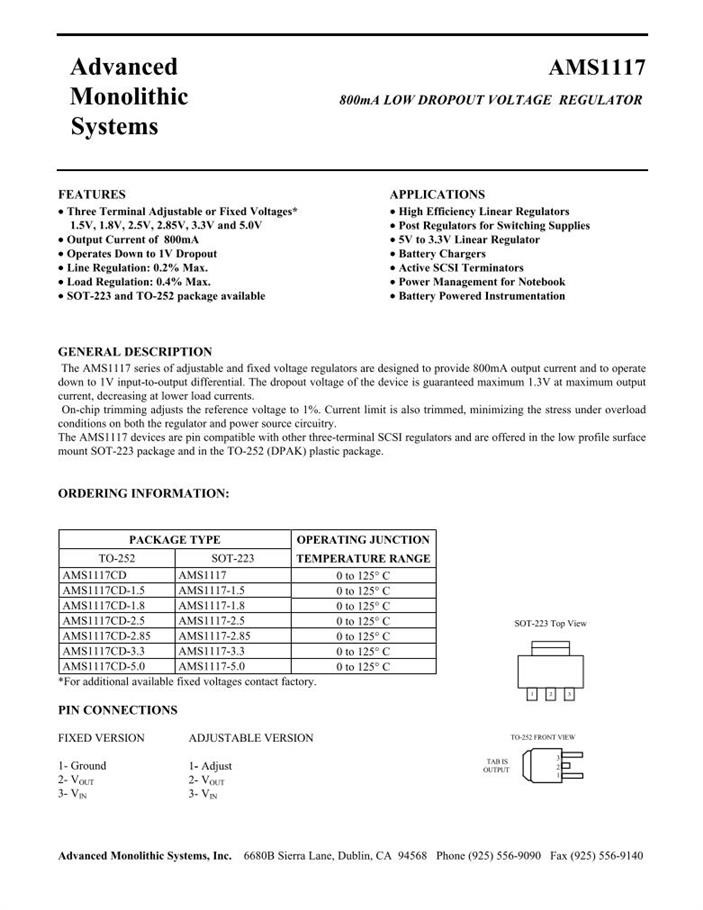
\includegraphics[width=\linewidth]{images/AMS.jpg}
\end{minipage}
\hfill
\begin{minipage}{0.6\textwidth}
Internetdokumentation. AMS1117 ADMOS | Alldatasheet. 800mA LOW DROPOUT VOLTAGE REGULATOR.
Online verfügbar unter http://www.advanced-monolithic.com/pdf/ds1117.pdf, zuletzt aktualisiert am 2024, zuletzt geprüft am 11.04.2024.
\\ \textbf{Kurzfassung:}
Das Datenblatt für den Spannungswandler AMS1117. Alle notwendigen Angaben, wie minimal/maximal Eingangs- zu Ausgangsspannung und Ausgangsstrom sind angegeben. Darüber hinaus sind noch viele weitere Informationen angegeben, wie z.B. Pin-Belegung, Temperaturverhalten, usw.
\end{minipage}
\textbf{Schlagwörter:}
3.3 V; 5 V; ALLDATASHEET; ARCHIVE; CATALOG; CHIP; DATABOOK; Datasheet; ELECTRONIC COMPONENT; IC; ISO COMPONENT; PDF; PDF DATASHEET; SEMICONDUCTOR; TRANSISTOR
\textbf{Bewertung:}
Das Datenblatt bietet alle notwendigen Angaben, welche benötigt werden. Optimal wäre noch ein zusätzlich Datenblatt in deutscher Übersetzung gewesen.
}

\STANDARD{Allegro (2022):}
{
\begin{minipage}{0.38\textwidth}
	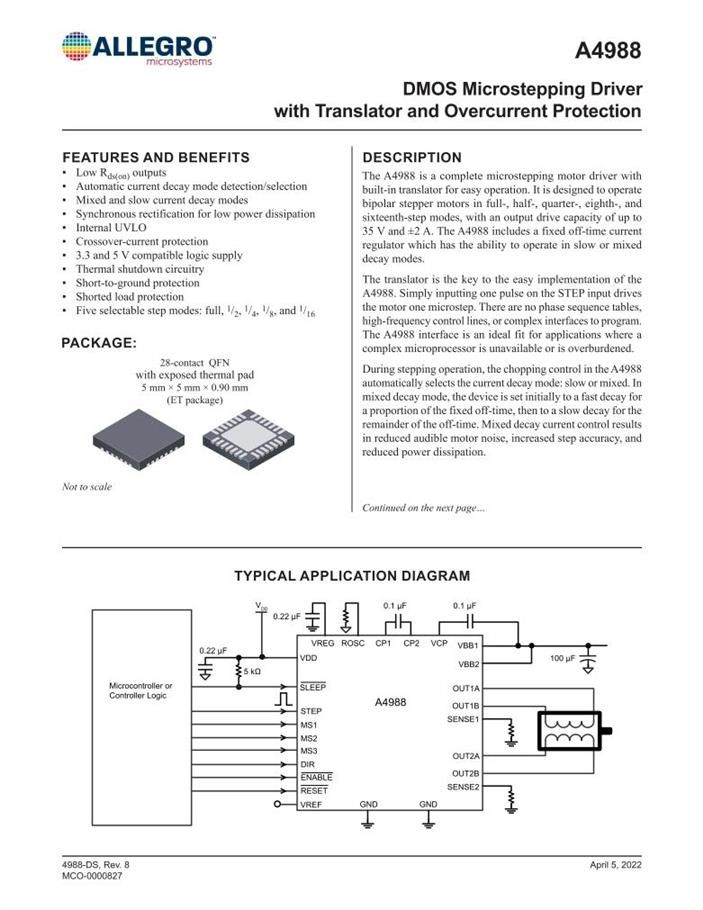
\includegraphics[width=\linewidth]{images/Allegro.jpg}
\end{minipage}
\hfill
\begin{minipage}{0.6\textwidth}
Internetdokumentation. A4988-Datasheet.
Online verfügbar unter https://www.allegromicro.com, zuletzt aktualisiert am 2022, zuletzt geprüft am 08.04.2024.
\\ \textbf{Kurzfassung:}
Datenblatt für die Schrittmotorsteuerung A4988. Es sind viele wichtige Informationen zur Inbetriebnahme des Schrittmotors angegeben: Die Logic Strom Versorgung ist mit 3.3 und 5 V möglich, 5 Schritt-Modis (step modes), Last-Versorgungsspannung mit bis zu 35 V und die Pin-Belegung.
\end{minipage}
\textbf{Schlagwörter:}
5 step modes; A4988; Motorsteuerung; Pin-Belegung; Schrittmotorsteuerung; Treiber
\\ \textbf{Bewertung:}
Das Datenblatt beinhaltet alle notwendigen Informationen für eine korrekte Inbetriebnahme.
}

\STANDARD{Arduino (2024):}
{
\begin{minipage}{0.38\textwidth}
	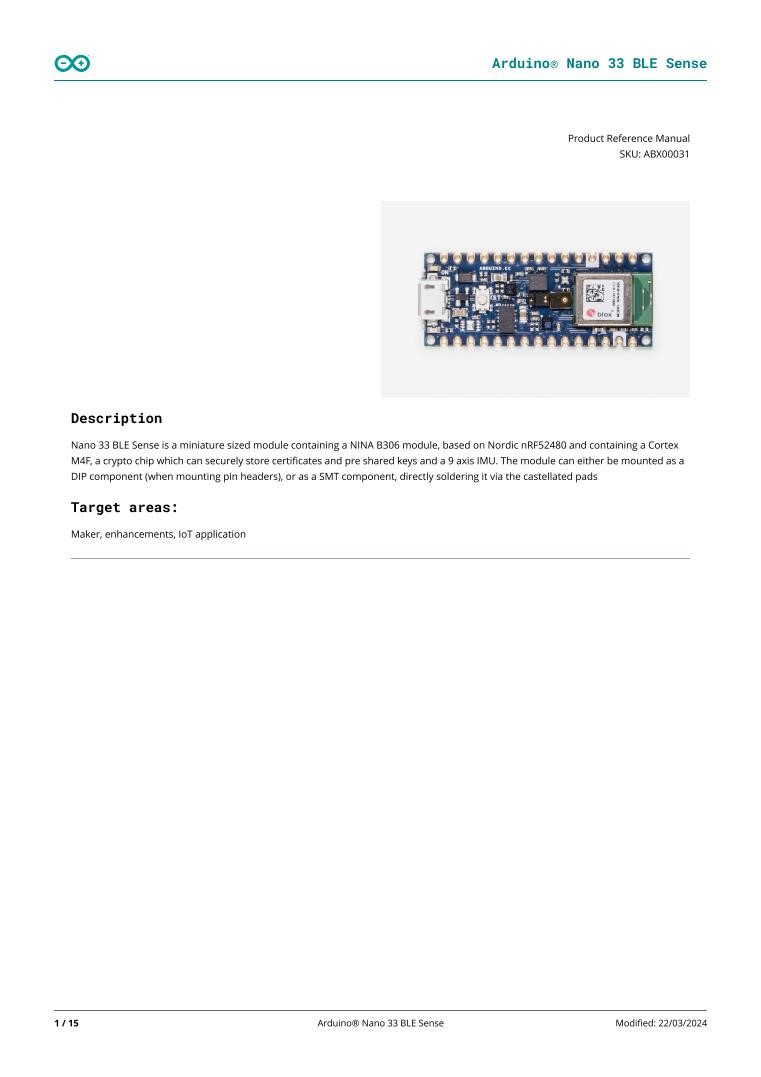
\includegraphics[width=\linewidth]{images/Arduino.jpg}
\end{minipage}
\hfill
\begin{minipage}{0.6\textwidth}
Internetdokumentation. ABX00031-Datasheet
zuletzt aktualisiert am 2024.
\\ \textbf{Kurzfassung:}
Eine detailliertes aber gut verständliches Handbuch zum Arduino Nano 33 BLE Sense. Mithilfe des Handbuches kann der Mikrocontroller fachgerecht in ein System integriert werden. Es wird außerdem ein kurzer Überblick aller im Arduino integrierten Sensoren gegeben.	
\end{minipage}
\textbf{Schlagwörter:}
Arduino; Arduino Nano 33 BLE Sense; Mikrocontroller; nicht 5 V verträglich; NRF52 Series; Pin-Belegung; Sensorik
\\ \textbf{Bewertung:}
Das Handbuch ist gut geeignet, um einen Überblick der Funktionen des Arduinos zu bekommen und es zu verdrahten. Jedoch sind die Funktionen der Sensoren und Peripherie-Geräte relativ kurz gehalten.
}

\STANDARD{Arduino IDE Dokumentation (2024) Mehrere Einträge:}
{
	
\includegraphics[width=0.38\linewidth]{images/IDE.jpg}
\begin{itemize}
	\item \textbf{Downloads. Arduino IDE 2.3.2:}
	Hg. v. Arduino. https://www.arduino.cc/en/software. Online verfügbar unter https://www.arduino.cc/en/software, zuletzt geprüft am 12.04.2024.
	\item \textbf{Installing a Board Package in the IDE 2:}
	Hg. v. Arduino. Online verfügbar unter https://docs.arduino.cc/software/ide-v2/tutorials/ide-v2-board-manager., zuletzt aktualisiert am 16.04.2024, zuletzt geprüft am 13.06.2024.
	\item \textbf{Installing Libraries:}
	Hg. v. Arduino. Online verfügbar unter https://docs.arduino.cc/software/ide-v2/tutorials/ide-v2-installing-a-library/, zuletzt aktualisiert am 12.02.2024, zuletzt geprüft am 12.04.2024.
	\item \textbf{loop:} Hg. v. Arduino. Online verfügbar unter https://docs.arduino.cc/software/ide-v2/tutorials/ide-v2-installing-a-library/, zuletzt aktualisiert am 12.02.2024, zuletzt geprüft am 12.04.2024.
	\item \textbf{setup:} Hg. v. Arduino. Online verfügbar unter https://www.arduino.cc/reference/en/language/structure/sketch/setup/, zuletzt geprüft am 12.04.2024.
\end{itemize}
\textbf{Kurzfassung:}
Die Arduino Software Dokumentation zur IDE ist eine Sammlung an Informationen, die Anwendern dabei hilft, sich mit der Arduino-Entwicklungsumgebung vertraut zu machen, ihre Programmierkenntnisse zu erweitern und Projekte zu realisieren. 
\\ \textbf{Schlagwörter:}
Arduino; Dokumentation; DIE; loop; setup; download; packages, libaries
\\ \textbf{Bewertung:}
Die Dokumentation auf der Arduino ist für Anfänger leicht zugänglich und bietet auch fortgeschrittenen Benutzern wertvolle Informationen und Unterstützung. Jedoch müssen gute Englischkenntnisse vorliegen, da keine Übersetzung in deutsch vorliegt.
}

\STANDARD{Arm (2020):}
{
\begin{minipage}{0.38\textwidth}
	\includegraphics[width=\linewidth]{images/Arm.jpg}
\end{minipage}
\hfill
\begin{minipage}{0.6\textwidth}
Internetdokument. Arm-Cortex-M4-Processor-Datasheet. Zuletzt aktualisiert am 2020.
\\ \textbf{Kurzfassung:}
Datenblatt für den Arm Cortex-M4 Prozessor.	
\\ \textbf{Schlagwörter:}
ArmCortex M4; Cortex-M4; Datasheet; Datenblatt; Prozessor
\\ \textbf{Bewertung:}
Ausführliches Datenblatt mit vielen weiteführenden Informationen zum Prozessor.
\end{minipage}
}

\STANDARD{Avago Technologies (2015):}
{
\begin{minipage}{0.38\textwidth}
	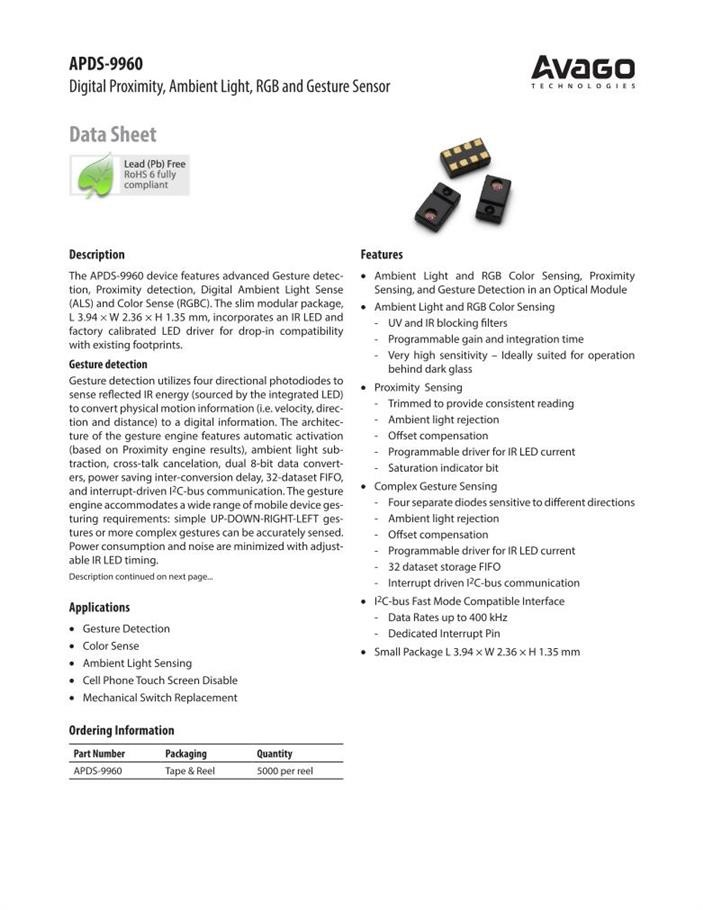
\includegraphics[width=\linewidth]{images/Avago.jpg}
\end{minipage}
\hfill
\begin{minipage}{0.6\textwidth}
Internetdokument. Datasheet - APDS-9960 - Digital Proximity, Ambient Light, RGB and Gesture Sensor. Zuletzt aktualisiert am 2015.
\\ \textbf{Kurzfassung:}
Datenblatt zum Näherungs-, Umgebungslicht-, Farb- und Gestensensor.
Weiterführende Informationen zum Sensor.
\\ \textbf{Schlagwörter:}
APDS-9960; Datasheet; Datenblatt; Farbsensor; Lichtsensor; Näherungssensor; Sensorik
\\ \textbf{Bewertung:}
Detailliertes Datenblatt zum APDS-9960 Sensor zur besseren Verständlichkeit.
\end{minipage}
}

\STANDARD{AZ-Delivery (2024):}
{
\begin{minipage}{0.38\textwidth}
	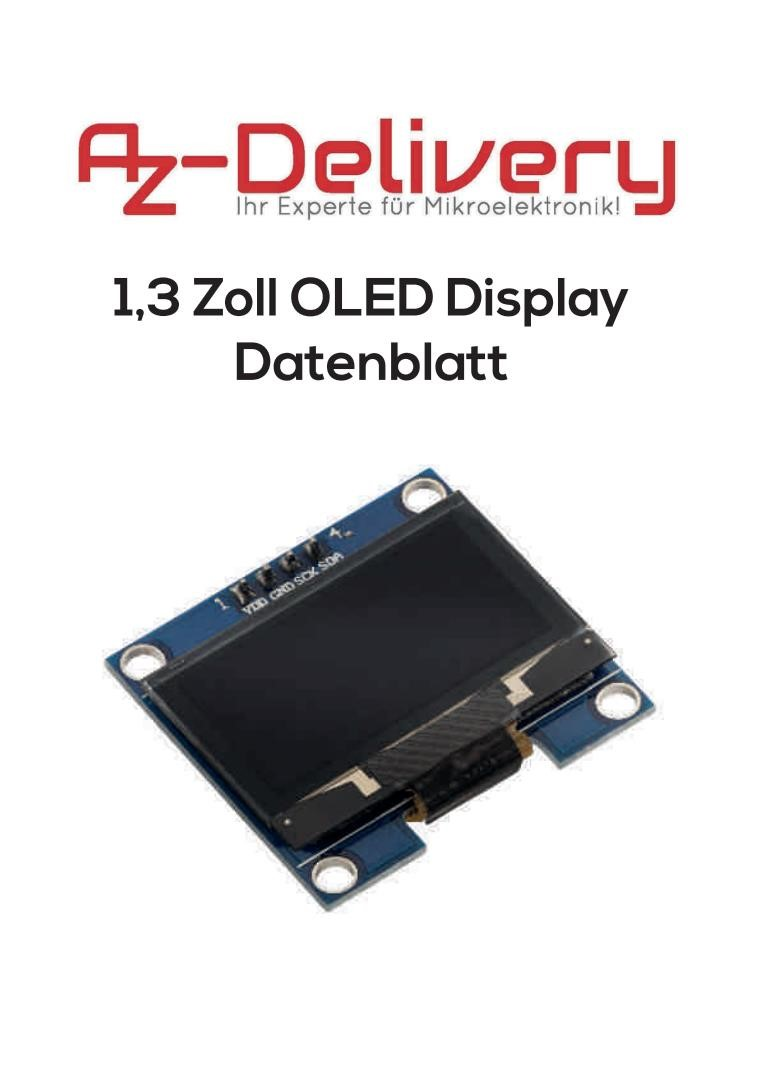
\includegraphics[width=\linewidth]{images/AZ.jpg}
\end{minipage}
\hfill
\begin{minipage}{0.6\textwidth}
Internetdokument. 1,3 Zoll OLED Display Datenblatt.
Hg. v. AZ-Delivery. Online verfügbar unter https://www.az-delivery.de/products/1-3zoll-i2c-oled-display, zuletzt geprüft am 26.04.2024.
\\ \textbf{Kurzfassung:}
Datenblatt zum OLED Display. Das Datenblatt enthält alle wichtigen Daten zur Integration des Displays und noch Informationen darüber hinaus.	
\\ \textbf{Schlagwörter:}
Bildschirm; Datasheet; Datenblatt; I2C; OLED
\\ \textbf{Bewertung:}
Gerade für die Systemintegration des Bildschirms, war das Datenblatt hilfreich, da alle Anschluss-Pins angegeben sind und die Bauteil Abmaße angegeben sind.
\end{minipage}
}

\STANDARD{Babiel, Gerhard (2023):}
{
Buch (Monographie). Elektrische Antriebe in der Fahrzeugtechnik. Lehr- und Arbeitsbuch.
5. Auflage. Wiesbaden, Heidelberg: Springer Vieweg.	
\begin{minipage}{0.38\textwidth}
	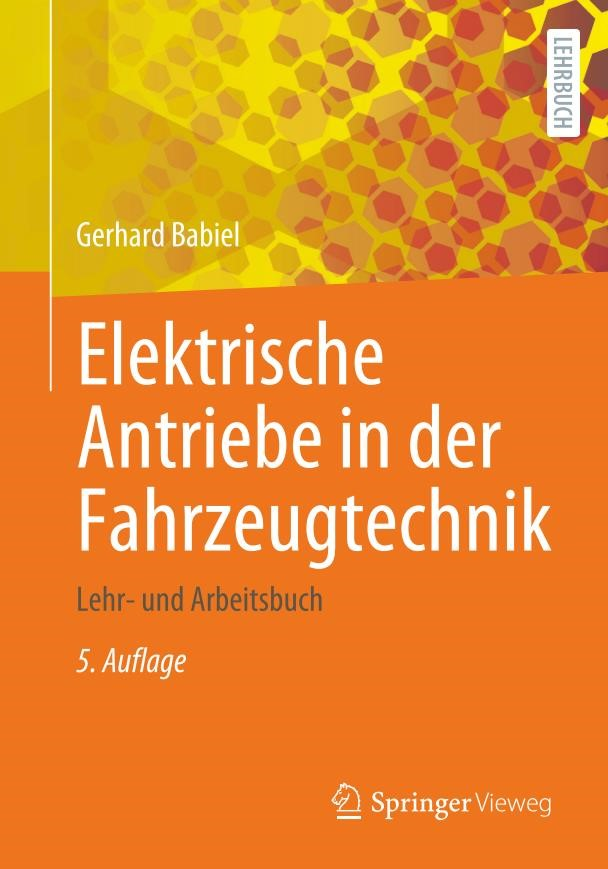
\includegraphics[width=\linewidth]{images/Babiel.jpg}
\end{minipage}
\hfill
\begin{minipage}{0.6\textwidth}
\textbf{Kurzfassung:}
Das Lehrbuch vermittelt die Grundlagen von der Energiegewinnung über die Energiewandlung bis zur Drehfeldmaschine und deren Anwendung in heutigen und vor allem zukünftigen Antriebssystemen. Zunächst werden aktuelle und zukünftige Energiequellen für Fahrzeugantriebe vorgestellt und miteinander verglichen. Darauf aufbauend werden elektrochemische Energiespeicher und -wandler wie die Wasserstoff-Brennstoffzelle behandelt. Es werden Gleichstrom-, Asynchron-, Synchron- und Linearmotor sowie Reluktanz-, Transversalfluss- und Digital-Motoren erklärt. Im letzten Kapitel werden Antriebssysteme am Beispiel einer E-Lok und der Magnetschwebebahn vorgestellt.
\end{minipage}
\textbf{Schlagwörter:}
Elektromotor; Mikroschrittverfahren; Positioniergenauigkeit; PWM; Schrittmotor
\\ \textbf{Bewertung:}
Das Lehrbuch ist ein umfassendes Lehrbuch für elektrische Antriebe. Für dieses Projekt wurden lediglich Auszüge aus dem Teil "Schrittmotoren" verwendet.
\\ \textbf{ISBN:}
978-3-658-40585-4
}

\STANDARD{Basler, Stefan (2016):}
{
Buch (Monographie). Encoder und Motor-Feedback-Systeme.
Wiesbaden: Springer Fachmedien Wiesbaden. Online verfügbar unter https://link.springer.com/book/10.1007/978-3-658-12844-9 \\
zuletzt geprüft am 11.04.2024.	\\
\begin{minipage}{0.38\textwidth}
	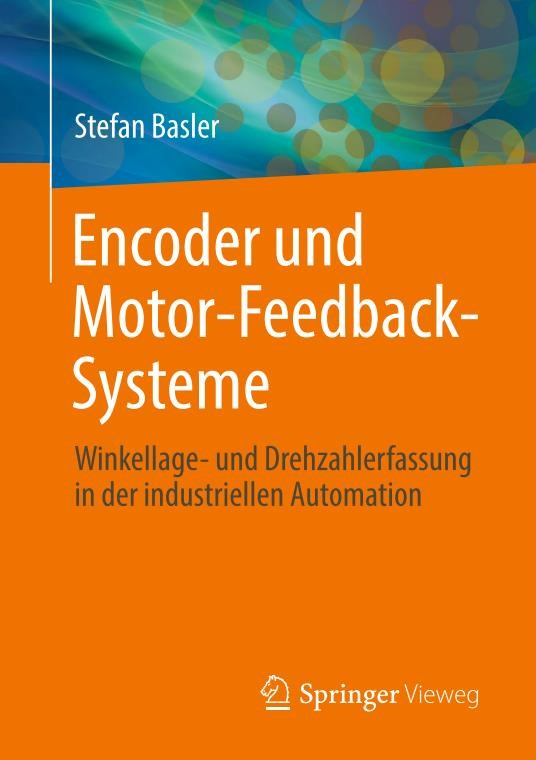
\includegraphics[width=\linewidth]{images/Basler.jpg}
\end{minipage}
\hfill
\begin{minipage}{0.6\textwidth}
\textbf{Kurzfassung:}
Das Buch gibt einen Einblick in die Theorie, die Sensorik, den Aufbau und die Anwendungen von Drehgebern. Encoder sind wichtige Komponenten in der Steuerungs- und Automatisierungstechnik, Motor-Feedback-Systeme in der modernen Antriebstechnik. Sie wandeln den Winkel zweier relativ zueinander drehbaren Objekte in ein elektrisches Signal um. Dies setzt man ein, um die Winkellage und die Drehzahl einer sich drehenden Achse zu erfassen. Das Wissen darüber hat eine große Bedeutung in der industriellen Automation und bei Servoantrieben.	
\end{minipage}
\textbf{Schlagwörter:}
Absolutdrehgeber; Automatisierungstechnik; Drehgeber; Encoder; Inkrementaldrehgeber; Regelungstechnik
\\ \textbf{Bewertung:}
Das Buch befasst sich sehr umfangreich mit der Thematik Drehgeber und Encoder. Mithilfe des Buches konnte die grundlegende Funktionsweise von Drehgebern errungen werden.
\\ \textbf{ISBN:}
978-3-658-12843-2
}

\STANDARD{Bernstein, Herbert (2018):}
{
Buch (Monographie). Elektrotechnik/Elektronik für Maschinenbauer. Einfach und praxisgerecht. 3., überarbeitete Auflage. \\Wiesbaden, Heidelberg: Springer Vieweg (Lehrbuch).\\
\begin{minipage}{0.38\textwidth}
	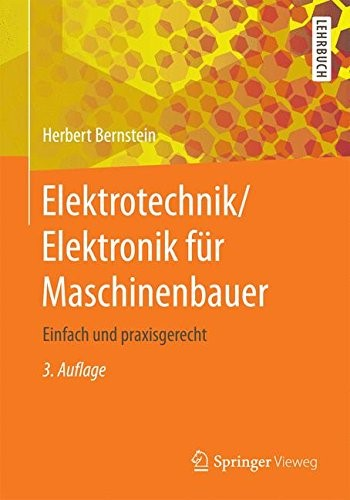
\includegraphics[width=\linewidth]{images/Bernstein.jpg}
\end{minipage}
\hfill
\begin{minipage}{0.6\textwidth}
\textbf{Kurzfassung:}
Dieses Lehrbuch behandelt anschaulich in Form von Beispielen oder Versuchen Gesetzmäßigkeiten beim Gleich- und Wechselstromkreis und erklärt die wichtigsten passiven Bauelemente. Es werden die wichtigsten elementaren Schaltungen zur elektrischen Messtechnik vorgestellt und die dazu benötigten analogen und digitalen Messgeräte. Grundlegende Bauelemente aus dem Bereich der Leistungshalbleiter werden mit ihren Anwendungen erklärt. Der Aufbau von Gleich-, Wechsel- und Drehstrommotoren mit Beispielen aus der Antriebstechnik wird verständlich dargestellt.
\end{minipage}
\textbf{Schlagwörter:}
Drehfeld; Elektromotor; Magnetfeld; Mikroschrittverfahren; Rotor; Schrittmotor; Stator
\\ \textbf{Bewertung:}
Herangezogen wurde dieses Buch für den Aufbau und der Funktionsweise von Schrittmotoren. Es konnte die bereits vorhanden Informationen ergänzen.
\\ \textbf{ISBN:}
978-3-658-20837-0
}

\STANDARD{Bernstein, Herbert (2020):}
{
Buch (Monographie). Mikrocontroller. Grundlagen der Hard- und Software der Mikrocontroller ATtiny2313, ATtiny26 und ATmega32.
2., aktualisierte und erweiterte Auflage.\\Wiesbaden, Heidelberg: Springer Vieweg (Lehrbuch). \\
\begin{minipage}{0.38\textwidth}
	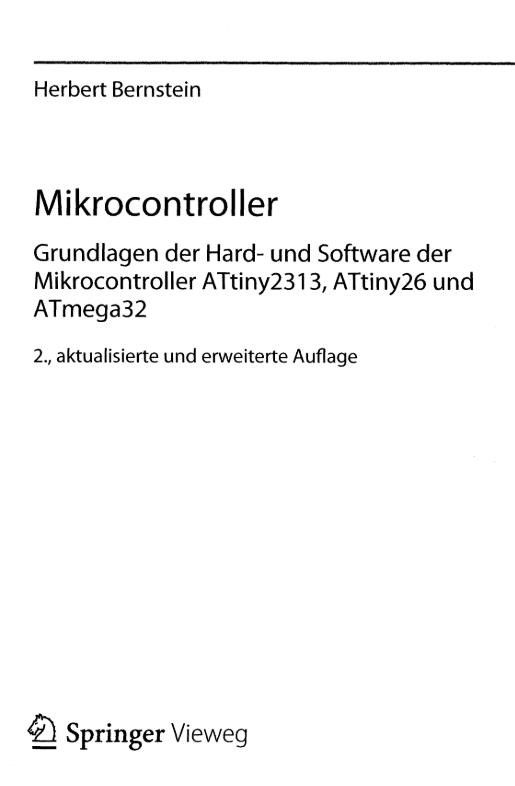
\includegraphics[width=\linewidth]{images/Bernstein2.jpg}
\end{minipage}
\hfill
\begin{minipage}{0.6\textwidth}
\textbf{Kurzfassung:}
Das Buch "Mikrocontroller Grundlagen der Hard- und Software" von Herbert Bernstein ist ein umfassendes Werk, das sich mit den Grundlagen der Mikrocontroller ATtiny2313, ATtiny26 und ATmega32 beschäftigt. Es bietet eine detaillierte Einführung in die Welt der Mikrocontroller und vermittelt sowohl theoretisches Wissen als auch praktische Anwendungen. So wird auch die Ansteuerung von Schrittmotoren mithilfe eines Mikrocontrollers behandelt.		
\end{minipage}
\textbf{Schlagwörter:}
ATmega32; ATtiny2313; ATtiny26; Bernstein; Grundlagen; I2C; IC; Mikrocontroller; Schrittmotorsteuerung
\\ \textbf{Bewertung:}
Besonders hilfreich war dieses Buch, um ein Verständnis von integrierten Schaltkreisen (I2C´s)  zu bekommen.
\\ \textbf{ISBN:}
978-3-658-30067-8
}

\STANDARD{Dieter Stotz (2019):}
{
Buch (Monographie). Computergestützte Audio- und Videotechnik. Multimediatechnik in der Anwendung. 3. Aufl. Berlin, Heidelberg: Springer Vieweg. Online verfügbar unter https://link.springer.com/book/10.1007/978-3-662-58873-4 \\zuletzt geprüft am 26.04.2024. \\
\begin{minipage}{0.38\textwidth}
	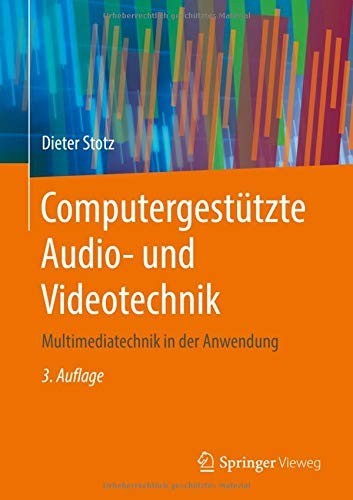
\includegraphics[width=\linewidth]{images/Stotz.jpg}
\end{minipage}
\hfill
\begin{minipage}{0.6\textwidth}
\textbf{Kurzfassung:}
Dieses Buch bietet eine leicht verständliche Einführung für moderne Audio- und Videotechnik im Verbund mit Computersystemen. Der Leser mit technischem Grundverständnis wird mit dem klar strukturierten Stoff einen leichten Einstieg in komplexe Zusammenhänge finden. Aus dem Inhalt: Tontechnik-Grundlagen, Abtastung und Digitalisierung, räumliches Hören, Methoden der Datenkompression, MIDI-Standard und -Signale, digitale Audiomesstechnik, Videotechnik-Grundlagen, hochauflösende Videotechnik und 3D-Technik, moderne Wiedergabesysteme (VR-Brille, OLED-Bildschirme), reales Raumsehen (Stand der Technik), Chromakeying, Schnittsysteme, Animationen, Dateienformate.	
\end{minipage}
\textbf{Schlagwörter:}
Dioden; Display; OLED
\\ \textbf{Bewertung:}
Das Buch wurde für herangezogen, um die grundlegende Funktionsweise und Vorzüge der OLED-Technik zu verstehen.
\\ \textbf{ISBN:}
978-3-662-58872-7
}

\STANDARD{Faulhaber Drive Systems (2020):}
{
\begin{minipage}{0.38\textwidth}
	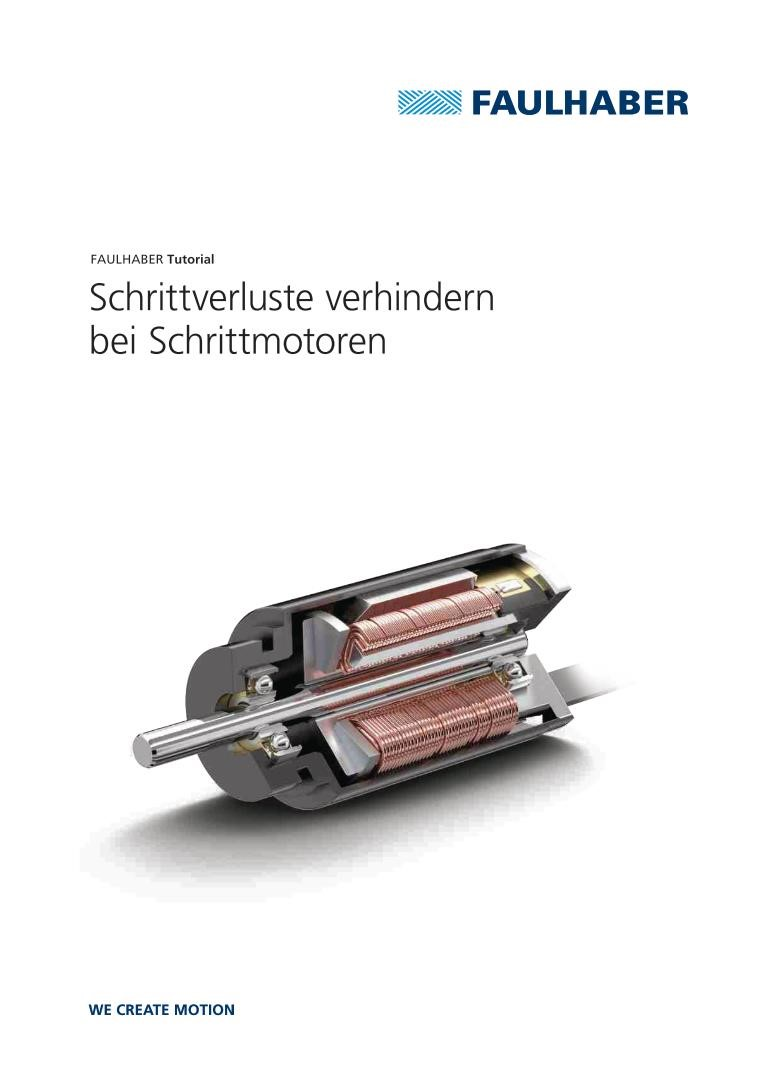
\includegraphics[width=\linewidth]{images/Faulhaber.jpg}
\end{minipage}
\hfill
\begin{minipage}{0.6\textwidth}
Internetdokument. Faulhaber Drive Systems (2020):
FAULHABER Tutorial. Schrittverluste verhindern bei Schrittmotoren.
Hg. v. DR. FRITZ FAULHABER GMBH \& CO. KG. Schönaich · Deutschland. Online verfügbar unter https://www.faulhaber.com/de/know-how/tutorials/schrittmotoren-tutorial-schrittverluste-verhindern-bei-schrittmotoren/, zuletzt geprüft am 14.05.2024.
\\ \textbf{Kurzfassung:}
Dieses Tutorial von Faulhaber gibt viele methodische Hinweise und Möglichkeiten, um Schrittverluste bei Schrittmotoren zu verhindern. Das Tutorial geht dabei strukturiert vor und führt durch die vier Punkte: Auswahl des Schrittmotors, Betriebsart, externe Kommutierungsfehler und externe Ereignisse.
\end{minipage}
\textbf{Schlagwörter:}
Faulhaber; Fehlerbehebung; Fehlerbilder; Lösung; Schrittmotor; Ursache
\\ \textbf{Bewertung:}
Das Tutorial war hilfreich bei der Auswahl und Inbetriebnahme des  Schrittmotors.
}

\STANDARD{Gehrke, Winfried; Winzker, Marco (2022):}
{
\begin{minipage}{0.38\textwidth}
	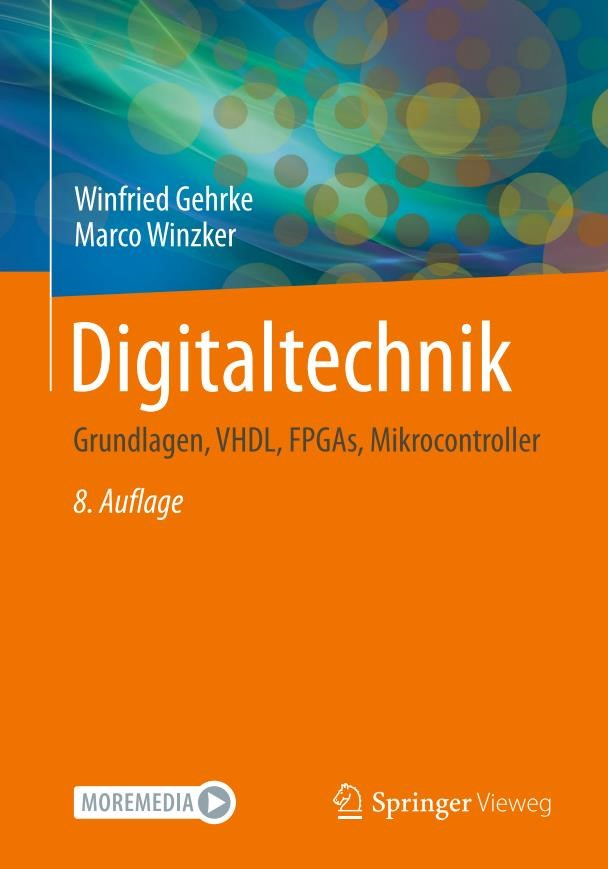
\includegraphics[width=\linewidth]{images/Gehrke.jpg}
\end{minipage}
\hfill
\begin{minipage}{0.6\textwidth}
Buch (Monographie). Digitaltechnik. Grundlagen, VHDL, FPGAs, Mikrocontroller.
8. Auflage. Berlin, Heidelberg: Springer Vieweg. Online verfügbar unter https://link.springer.com/book/10.1007/978-3-662-63954-2.
\\ \textbf{Kurzfassung:}
Moderne Digitaltechnik, umfassend und kompakt: Dieses Lehr- und Übungsbuch spannt den Bogen von den Grundlagen der Digitaltechnik über den Entwurf mit VHDL und Komponenten digitaler Systeme bis zu modernen Mikrocontrollern der STM32-Serie.	
\end{minipage}
\textbf{Schlagwörter:}
ArmCortex; DMA; I2C; IC; Mikrocontroller
\\ \textbf{Bewertung:}
Dieses Buch war besonders als Nachschlagewerk von Fachbegriffen im Bereich der Mikrocontroller hilfreich.
\\ \textbf{ISBN:}
9783662639535
}

\STANDARD{Hagl, Rainer (2021):}
{
Buch (Monographie). Elektrische Antriebstechnik.
3., überarbeitete und erweiterte Auflage. München: Hanser. \\
\begin{minipage}{0.38\textwidth}
	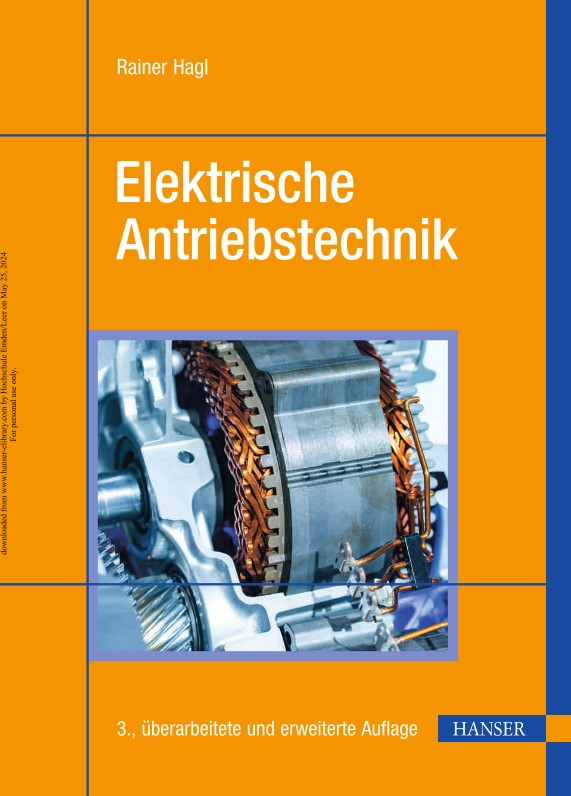
\includegraphics[width=\linewidth]{images/Hagl.jpg}
\end{minipage}
\hfill
\begin{minipage}{0.6\textwidth}
\textbf{Kurzfassung:}
Dieses Lehrbuch bietet einen Überblick über den Aufbau und die Wirkungsweise von elektrischen Antrieben. Es zeigt, wie Antriebe bezüglich Produktivität, Kosten, Bauraum und Energieeffizienz optimiert werden können. Zu Beginn des Buches werden die Anforderungen an elektrische Antriebe sowie deren Hauptunterscheidungsmerkmale erläutert. Die Aufgaben einzelner Komponenten wie Motor, mechanische Übertragungselemente oder Positionsmessgeräte werden beschrieben, Grundbeziehungen herausgearbeitet und Begriffe zum Thema Produktinformation erklärt. Im Hauptteil werden Motoren in Antrieben von Produktionsmaschinen erläutert.
\end{minipage}
\textbf{Schlagwörter:}
bipolar; Halbschritt; Hybridschrittmotor; Magnetfeld; Mikroschrittverfahren; Positioniergenauigkeit; Reluktanzschrittmotor, Vollschritt; Rotor; Schrittmotor; Stator; unipolar
\\ \textbf{Bewertung:}
Dieses Buch wurde für grundlegende Funktionsweise, den Aufbau und die verschiedenen Bauformen von Schrittmotoren herangezogen. Die Ausführungen sind übersichtlich und gut verständlich geschrieben.
\\ \textbf{ISBN:}
978-3-446-46572-5
}

\STANDARD{Global Electric Motor Solution LLC:}
{
\begin{minipage}{0.38\textwidth}
	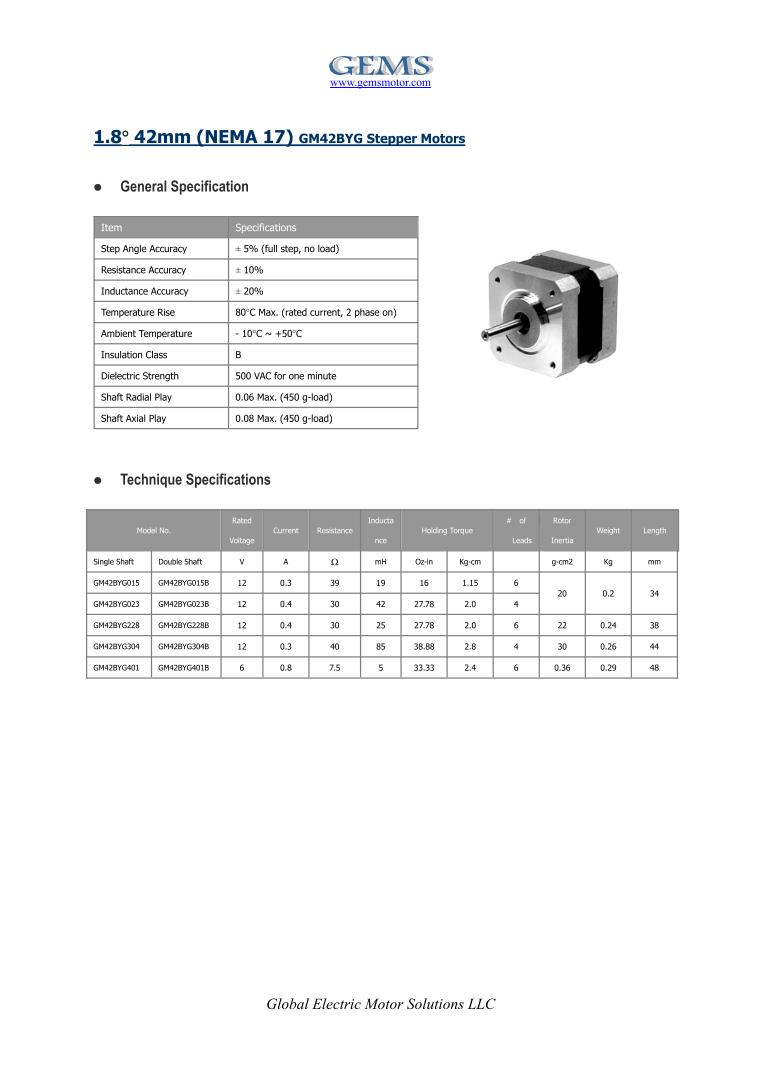
\includegraphics[width=\linewidth]{images/Gems.jpg}
\end{minipage}
\hfill
\begin{minipage}{0.6\textwidth}
Internetdokument. NEMA 17, 1.8° 42mm GM42BYG Stepper Motors. Online verfügbar unter https://gemsmotor.com/stepper/nema17-stepper-motor.pdf, zuletzt geprüft am 19.06.2024.
\\ \textbf{Kurzfassung:}
Datenblatt zum NEMA 17, 1.8° 42mm GM42BYG Schrittmotor
\\ \textbf{Schlagwörter:}
1.8°; 12 V; 42mm; Datasheet; Datenblatt; GM42BYG; NEMA 17; Schrittmotor; Stepper Motors
\end{minipage}
\textbf{Bewertung:}
Sehr einfach gehaltenes Datenblatt. Es wurde eine Beschreibung der genauen  Pin-Belegung vermisst. Außerdem ist kein Erstelldatum angegeben.
}

\STANDARD{Lienig, Jens; Dietrich, Manfred (Hg.) (2012):}
{
\begin{minipage}{0.38\textwidth}
	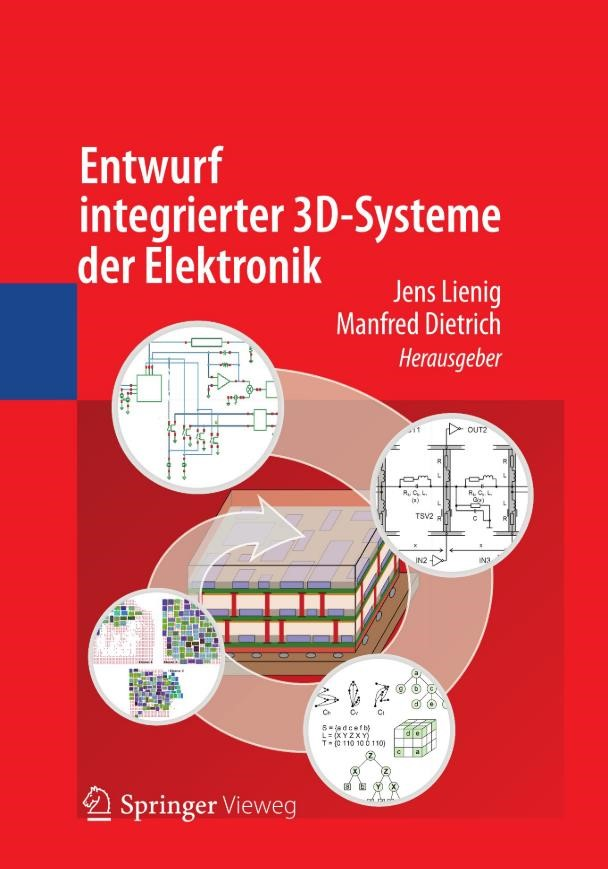
\includegraphics[width=\linewidth]{images/Lienig.jpg}
\end{minipage}
\hfill
\begin{minipage}{0.6\textwidth}
Buch (Sammelwerk). Entwurf integrierter 3D-Systeme der Elektronik.
Berlin, Heidelberg: Springer Vieweg.
\\ \textbf{Kurzfassung:}
Nach einer Einführung in 3D-Systeme (Teil I) mit den sich ergebenden neuen Anwendungsmöglichkeiten wird detailliert auf die beiden wesentlichen Abschnitte des Entwurfs - Modellierung und Simulation (Teil II) sowie Layoutentwurf (Teil III) - eingegangen. Die Behandlung der Probleme mit zugehörigen Lösungsansätzen erfolgt dabei entsprechend des Entwurfsflusses, d. h. in der Reihenfolge ihrer Bearbeitung.
\end{minipage}
\textbf{Schlagwörter:}
3D-Baufruppe; 3D-Entwurf; Design and construction; Integrated circuits; Integrationstechnologien; Modellierung; Simulation; System-in-Package; Three-dimensional integrated circuits
\\ \textbf{Bewertung:}
Dieses Buch wurde zusätzlich herangezogen, um die IC- und I2C-Kommunikation bei Mikrocontrollern zu verstehen.
\\ \textbf{ISBN:}
978-3-642-30572-6
}

\STANDARD{Meanwell (2019):}
{
\begin{minipage}{0.38\textwidth}
	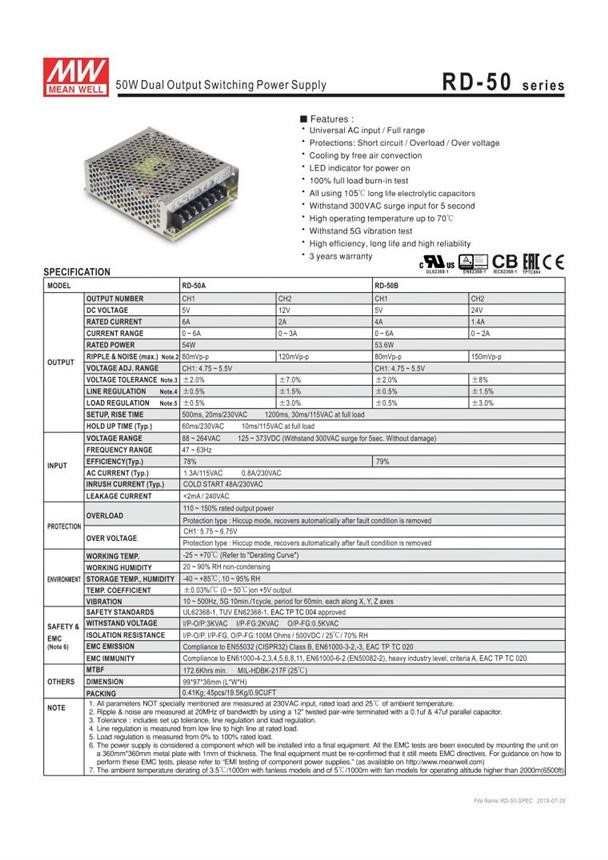
\includegraphics[width=\linewidth]{images/Meanwell.jpg}
\end{minipage}
\hfill
\begin{minipage}{0.6\textwidth}
Internetdokument. RD-50-20190729.cdr.
Online verfügbar unter https://cdn-reichelt.de/documents/datenblatt/D500/RD-50-DS-EN.PDF, zuletzt geprüft am 11.04.2024.
\\ \textbf{Kurzfassung:}
Datenblatt zum Schaltnetzteil RD-50 A.
\\ \textbf{Schlagwörter:}
12 V; 24 V; 5 V; RD-50 A; Schaltnetzteil; technische Zeichnung
\end{minipage}
\textbf{Bewertung:}
Das Datenblatt enthält alle wichtigen Informationen zur Inbetriebnahme. Hilfreich war zudem die technische Zeichnung des Netzteils für die Gehäusekonstruktion.
}

\STANDARD{Mentor (2024):}
{
\begin{minipage}{0.38\textwidth}
	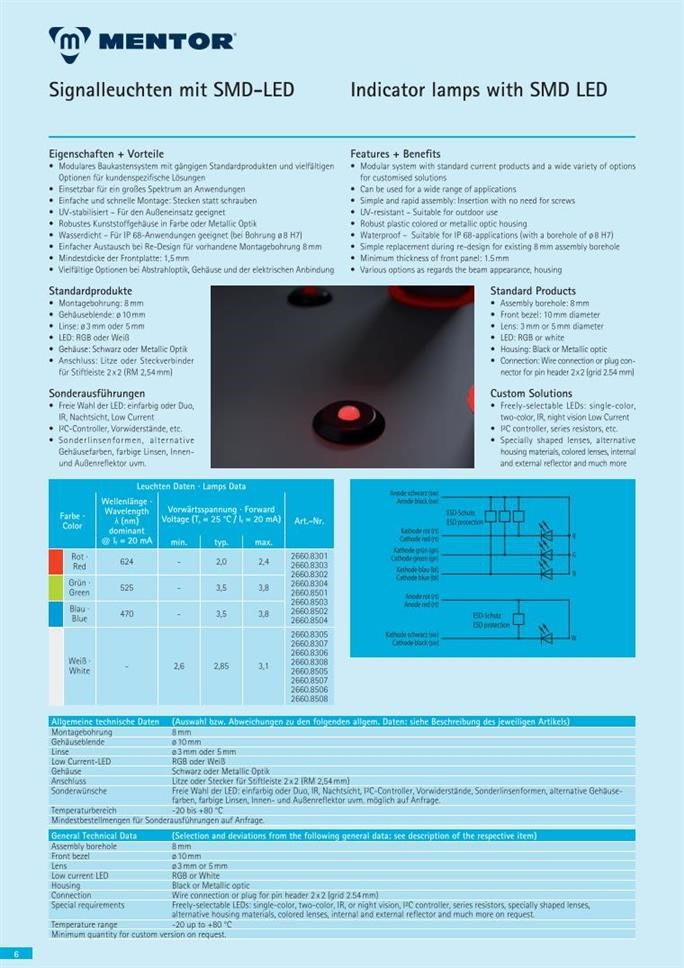
\includegraphics[width=\linewidth]{images/Mentor.jpg}
\end{minipage}
\hfill
\begin{minipage}{0.6\textwidth}
Internetdokument. SIGNALLEUCHTENSMD-LED-Datenblatt.
Online verfügbar unter https://www.mentor.de.com/bauelemente/product/2660-8301, zuletzt aktualisiert am 2024, zuletzt geprüft am 10.04.2024.	
\\ \textbf{Kurzfassung:}
Datenblatt für die  Signalleuchte von Mentor.
\\ \textbf{Schlagwörter:}
LED; Mentor; Signalleuchte; SMD-LED
\\ \textbf{Bewertung:}
Alle nötigen Spezifikationen sind angegeben. War besonders für die Konstruktion des Gehäuse hilfreich.
\end{minipage}
}

\STANDARD{Meroth, Ansgar; Sora, Petre (2021):}
{
Buch (Monographie). Sensornetzwerke in Theorie und Praxis.
Wiesbaden: Springer Fachmedien Wiesbaden. Online verfügbar unter https://link.springer.com/book/10.1007/978-3-658-31709-6.
 \\
\begin{minipage}{0.38\textwidth}
	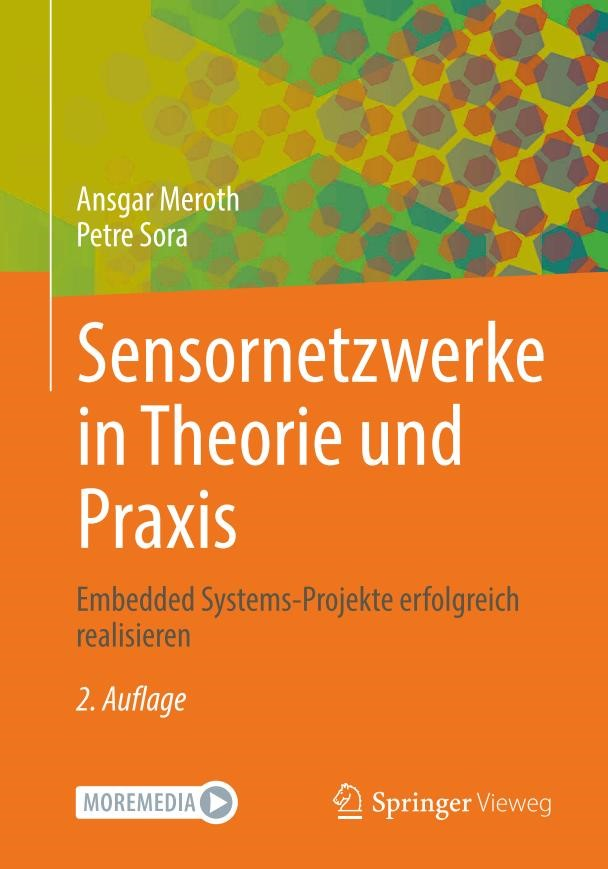
\includegraphics[width=\linewidth]{images/Meroth.jpg}
\end{minipage}
\hfill
\begin{minipage}{0.6\textwidth}
\textbf{Kurzfassung:}
Das Buch bildet eine  Grundlage für das Verständnis des Internet of Things, indem es einen Einblick in Vernetzungsprotokolle aus der Mikrocontrollerwelt bietet und Sensoren und andere Bausteine, sowie deren Einsatz und Programmierung vorstellt. Alle gezeigten Konzepte werden durch praktische Schaltungs- und Programmierbeispiele illustriert. Daneben stehen den Lesern offene Bibliotheken für die Ansteuerung der im Buch präsentierten Bauteile auf der Verlagshomepage zum Herunterladen bereit. Die zweite Auflage beinhaltet einige neue Bausteine, im Bereich der Netzwerke, eine Beschreibung der Funktionsprinzipien einiger Sensoren sowie weitere Tipps zum Programmieren.
\end{minipage}
\textbf{Schlagwörter:}
Arduino; Elektrotechnik; Embedded Systems; I2C; Mikrocontroller
\\ \textbf{Bewertung:}
Das Buch enthielt eine sehr gut verständliche Erklärung zum I2C-Kommunikationsprotokoll.
\\ \textbf{ISBN:}
978-3-658-31708-9
}

\STANDARD{Nordic Semiconductor. Mehrere Einträge:}
{
Internetdokument. SIGNALLEUCHTENSMD-LED-Datenblatt. \\
\begin{minipage}{0.38\textwidth}
	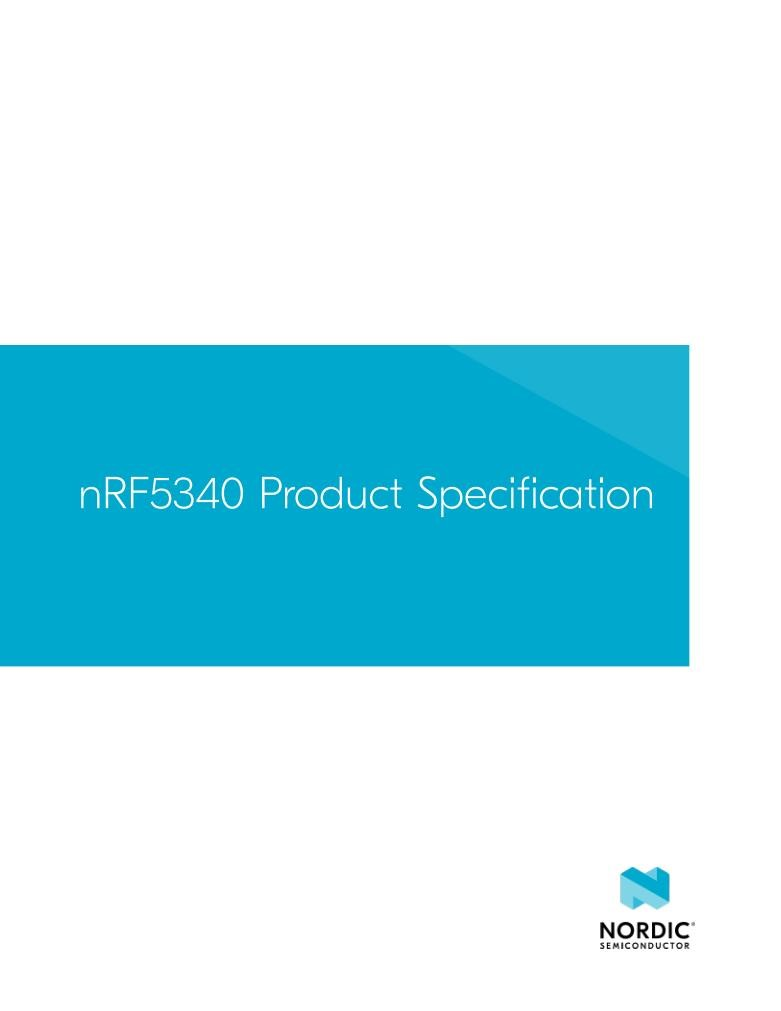
\includegraphics[width=\linewidth]{images/Nordic.jpg}
\end{minipage}
\hfill
\begin{minipage}{0.6\textwidth}
\begin{itemize}
	\item nRF5340 Product Specification. QSPI - Quad serial peripheral interface (2023)
	\item nRF52840 Product Specification Memory (2024)
	\item nRF52840 Product Specification 2 (2024)
	\item nRF9161 Product Specification. Cryptocell-ARM TrustZone CryptoCell 310 (2024)
\end{itemize}
Online verfügbar unter https://infocenter.nordicsemi.com, zuletzt geprüft am 09.04.2024.
\end{minipage}
\textbf{Kurzfassung:}
Ausführliche Dokumentation der nRF5340, nRF52840 und nRF9161 Produkt Spezifikationen.
\\ \textbf{Schlagwörter:}
NRF52 Series; Peripherals; QSPI; ArmCortex M4; Bluetooth 5; NFT; AAR; AES; CCM; ECB
\\ \textbf{Bewertung:}
Wurde nur in Auszügen und als Nachschlagewerk genutzt. 
}

\STANDARD{Petr Filipi; Arduino Tech Support Team (Dozie) (2022):}
{
\begin{minipage}{0.38\textwidth}
	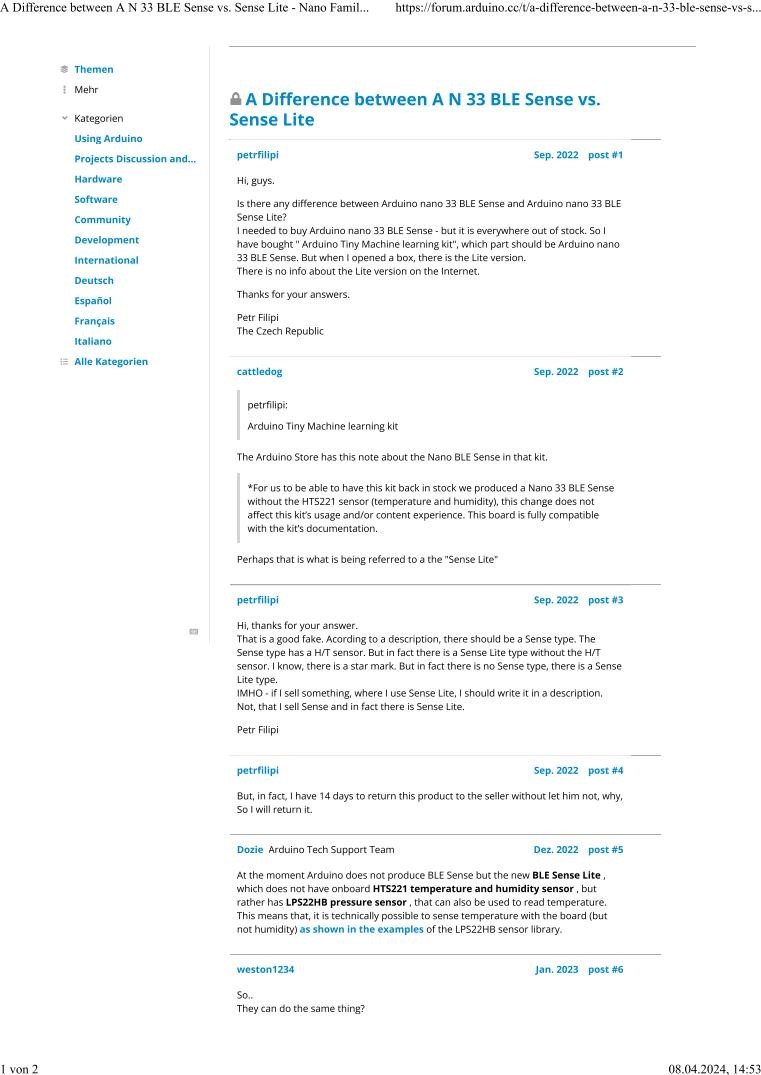
\includegraphics[width=\linewidth]{images/Filipi.jpg}
\end{minipage}
\hfill
\begin{minipage}{0.6\textwidth}
Internetdokument. Difference between A33BLESense and SenseLite. A Difference between A N 33 BLE Sense vs. Sense Lite. Online verfügbar unter https://forum.arduino.cc/t/a-difference-between-a-n-33-ble-sense-vs-sense-lite/1030305, zuletzt aktualisiert am 30.06.2023, zuletzt geprüft am 08.04.2024.
\\ \textbf{Kurzfassung:}
Forum Beitrag der bestätigt, dass der Arduino 33 BLE Sense Lite keinen HTS221 Temperatur- und Feuchtigkeits-Sensor hat.
\end{minipage}
\textbf{Schlagwörter:}
Arduino; Arduino Nano 33 BLE Sense; Arduino Nano 33 BLE Sense Lite; Forum; HTS221; Learning Kit
\\ \textbf{Bewertung:}
Leider gibt es kein zusätzliches Datenblatt für den Arduino 33 BLE Sense Lite. Zudem keinen zusätzlichen Vermerk des fehlenden Sensors.
}

\STANDARD{Schröder, Dierk; Kennel, Ralph (2021):}
{
\begin{minipage}{0.38\textwidth}
	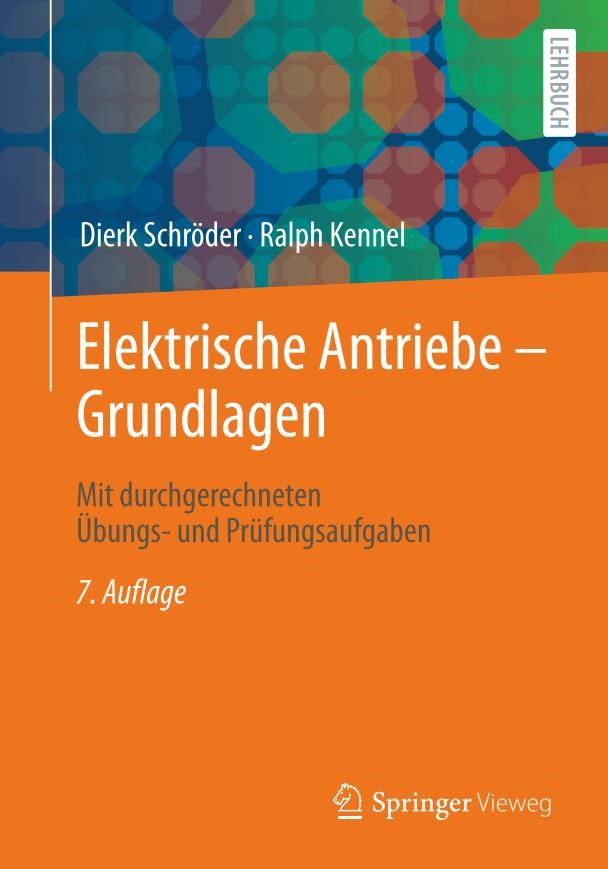
\includegraphics[width=\linewidth]{images/Schroeder.jpg}
\end{minipage}
\hfill
\begin{minipage}{0.6\textwidth}
Buch (Monographie). Elektrische Antriebe – Grundlagen. Berlin, Heidelberg: Springer Berlin Heidelberg.	
\\ \textbf{Kurzfassung:}
Dieses Werk bietet einen Einstieg in das Gebiet der elektrischen Antriebstechnik. Ausgehend von den mechanischen und elektromagnetischen Grundlagen, werden die Antriebskonzepte sowohl mit Gleichstrommaschinen als auch mit Asynchron- und Synchronmaschinen erläutert. Systemgleichungen, Signalflusspläne und Regelungsvarianten werden vorgestellt und diskutiert. Das Lehrbuch stellt abschließend Übungs- und Prüfungsaufgaben mit Lösungen zur Verfügung.
\end{minipage}
\textbf{Schlagwörter:}
Antriebstechnik; Automatisierungstechnik; Betriebsarten; bipolar; elektrische Antriebe; elektrische Energietechnik; elektrische Maschinen; Elektrotechnik; Hybridschrittmotor; Permanentmagneterregter Schrittmotor; Regelungstechnik; Reluktanzschrittmotor; Rotor; Schrittmotor; Selbsthaltemoment; Stator; unipolar
\\ \textbf{Bewertung:}
Dieses Buch wurde als Quelle für die Beschreibung des Schrittmotors verwendet. Die Ausführungen sind sehr Ausführlich, ergänzte somit gut die restliche Literatur zum Schrittmotor.
\\ \textbf{ISBN:}
978-3-662-63100-3
}

\STANDARD{Simac Electronics GmbH (2019):}
{
\begin{minipage}{0.38\textwidth}
	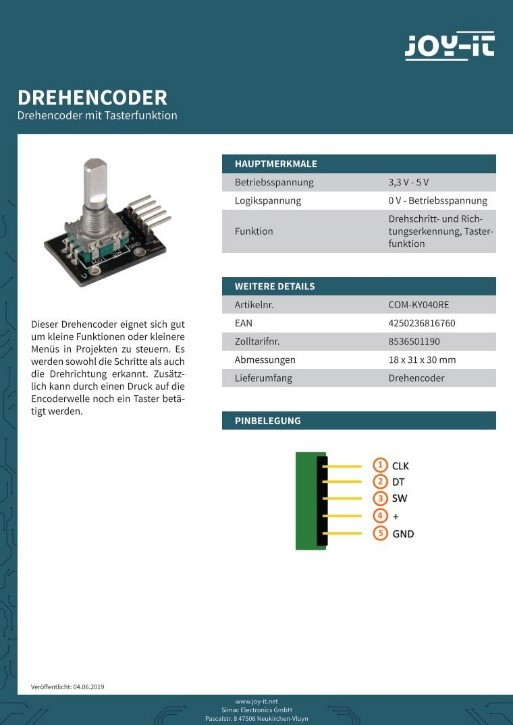
\includegraphics[width=\linewidth]{images/Simac.jpg}
\end{minipage}
\hfill
\begin{minipage}{0.6\textwidth}
Internetdokument. COM-KY040RE-Datenblatt. Drehencoder mit Tasterfunktion.
Online verfügbar unter www.joy-it.net, zuletzt aktualisiert am 2019, zuletzt geprüft am 11.04.2024.
\\ \textbf{Kurzfassung:}
Datenblatt zum Drehencoder. Betriebsspannung, Abmessungen und Pinbelegung sind angegeben.
\\ \textbf{Schlagwörter:}
3.3 V; 5 V; Abmessungen; Datenblatt; Drehencoder; Taster-Funktion
\end{minipage}
\textbf{Bewertung:}
Übersichtliches Datenblatt mit allen notwendigen Informationen.
}

\STANDARD{STMICROELECTRONICS (2015):}
{
\begin{minipage}{0.38\textwidth}
	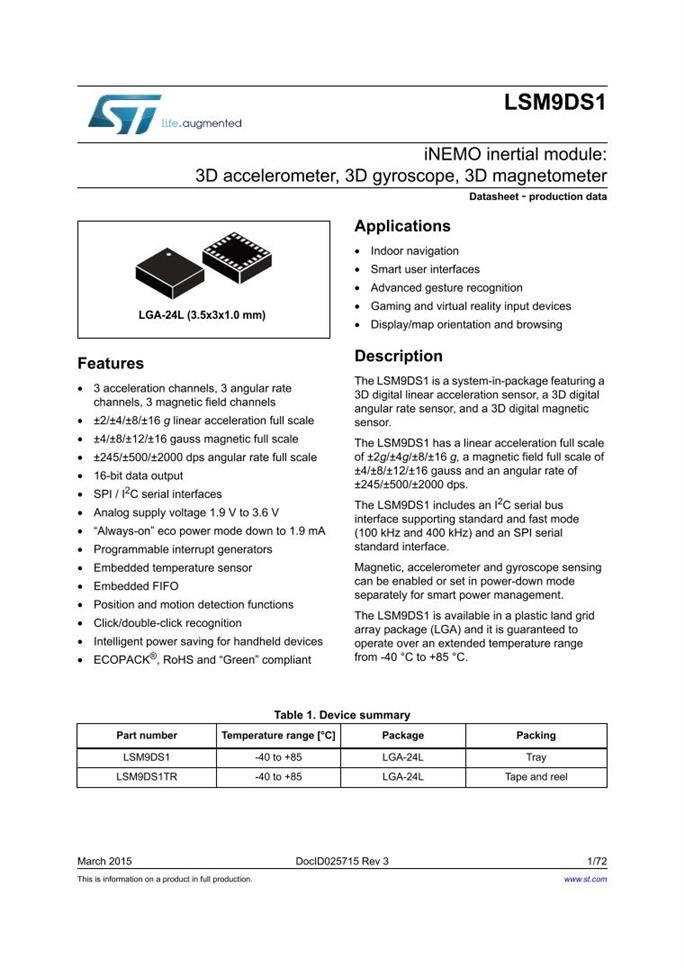
\includegraphics[width=\linewidth]{images/STM.jpg}
\end{minipage}
\hfill
\begin{minipage}{0.6\textwidth}
Internetdokument. Datasheet - LSM9DS1- iNEMO inertial module: 3D accelerometer, 3D gyroscope, 3D magnetometer.	Hg. v. STMICROELECTRONICS. Online verfügbar unter https://www.st.com/en/mems-and-sensors/lsm9ds1.html, zuletzt aktualisiert am 2015.
\\ \textbf{Kurzfassung:}
Datenblatt zum LSM9DS1 (9-Achs-IMU). Sehr umfangreiches Datenblatt. Die wichtigsten Informationen sind auf der ersten Seite kurz zusammengefasst.
\\ \textbf{Schlagwörter:}
Beschleunigungsmesser; Datasheet; Datenblatt; Gyroskop; I2C; IMU; LSM9DS1; Magnetometer; Product Development; Specification; SPI; System-in-Package; Technical Literature
\end{minipage}
\textbf{Bewertung:}
Alle möglichen Informationen der IMU konnten hier entnommen werden. Auch Informationen zur weiteren Systemintegration der IMU, wie z.B. für die I2C-Kommunikation sind hier angegeben.
}

\STANDARD{STMICROELECTRONICS (2017):}
{
\begin{minipage}{0.38\textwidth}
	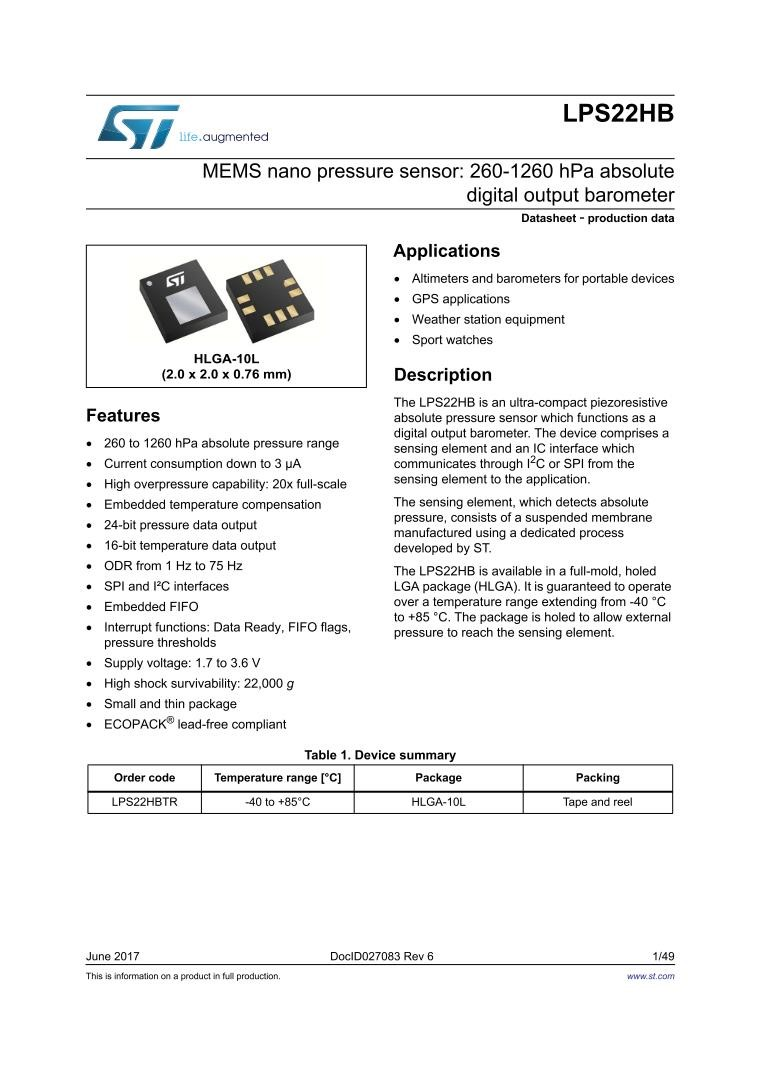
\includegraphics[width=\linewidth]{images/STM2.jpg}
\end{minipage}
\hfill
\begin{minipage}{0.6\textwidth}
Internetdokument. Datasheet - LPS22HB-MEMS nano pressure sensor: 260-1260 hPa absolute digital output barometer.
Hg. v. STMICROELECTRONICS. Online verfügbar unter https://www.st.com/en/mems-and-sensors/lps22hb.html, zuletzt aktualisiert am 2017.
\\ \textbf{Kurzfassung:}
Datenblatt zum LPS22HB Barometrischen Drucksensor. Sehr umfangreiches Datenblatt. Die wichtigsten Informationen sind auf der ersten Seite kurz zusammengefasst.
\end{minipage}
\textbf{Schlagwörter:}
027083; Barometrischer Drucksensor; Datasheet; Datenblatt; I2C; LPS22HB; Product Development; Specification; Technical Literature
\\ \textbf{Bewertung:}
Alle möglichen Informationen des Drucksensors konnten hier entnommen werden. Auch Informationen zur weiteren Systemintegration des Sensors, wie z.B. für die I2C-Kommunikation sind hier angegeben.
}

\STANDARD{STMICROELECTRONICS (2021):}
{
\begin{minipage}{0.38\textwidth}
	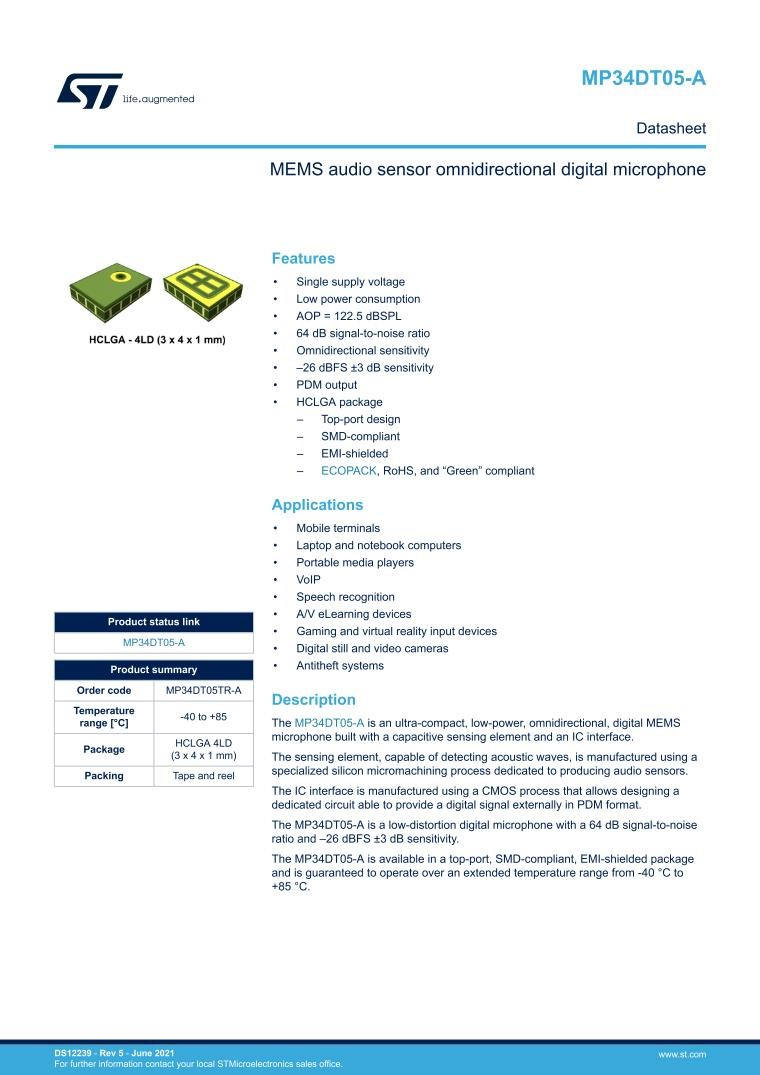
\includegraphics[width=\linewidth]{images/STM3.jpg}
\end{minipage}
\hfill
\begin{minipage}{0.6\textwidth}
Internetdokument. Datasheet - MP34DT05-A - MEMS audio sensor omnidirectional digital microphone. Hg. v. STMICROELECTRONICS.
\\ \textbf{Kurzfassung:}
Datenblatt zum MP34DT05-A Digitalen Mikrophone. Das MP34DT05-A ist ein ultrakompaktes, stromsparendes, omnidirektionales, digitales MEMS-Mikrofon mit einem kapazitiven Sensorelement und einer IC-Schnittstelle.
\\ \textbf{Schlagwörter:}
Datasheet; Datenblatt; I2C; Mikrofon; MP34DT05-A
\end{minipage}
\textbf{Bewertung:}
Ausführliches Datenblatt mit allen wichtigen Informationen.
}

\STANDARD{Weber, Irene (2024):}
{
Buch (Monographie). VBA für Office-Automatisierung und Digitalisierung.
Wiesbaden: Springer Fachmedien Wiesbaden.
 \\
\begin{minipage}{0.38\textwidth}
	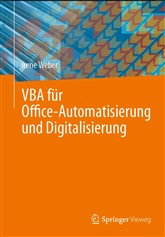
\includegraphics[width=\linewidth]{images/Weber.jpg}
\end{minipage}
\hfill
\begin{minipage}{0.6\textwidth}
\textbf{Kurzfassung:}
VBA bietet das Potenzial, effektive Digitalisierungslösungen mit geringem Aufwand zu realisieren. “VBA für Office-Automatisierung und Digitalisierung" zeigt mit vielen Codebeispielen die Automatisierung von Excel, Word, Outlook, PowerPoint, SAP ERP und SOLIDWORKS und das Zusammenwirken dieser Systeme. Auch Webservices und Rest APIs werden mit VBA angesprochen und erschließen interessante Möglichkeiten bis hin zu KI. Das Buch erläutert wichtige Konzepte und gibt viele Tipps, um VBA-Anwendungen mit einfachen Mitteln unternehmenstauglich und administrierbar zu gestalten.
\end{minipage}
\textbf{Schlagwörter:}
Computer Aided Design (CAD); Digitalisierung; End-User Computing; Fehlerbehebung; Office Programmierung; SolidWorks; VBA; Visual basic for applications
\\ \textbf{ISBN:}
978-3-658-42716-0
}